\chapter{RNA Motifs}
\label{motifs} 
\bibliographystyle{nar}
As mentioned  in Chapter 2 until  now the most  common perspectives on
RNA motif recognition  and discovery have been chemical,  based on the
atoms  and bonds.  The  rigid-body based  perspective involved  in the
interactions and the internal parameters taht describe the 3D folds on
RNA motifs, by contrast, has  been rather unexplored.  In this chapter
we address two main questions:

\begin{enumerate}
\item{Can the  geometric, rigid-block description  of base-pairing and
  base-stacking help to define RNA structural motifs?}
\item{Can quantities derived from the 3DNA software package be used to
  perform an automated search for  known RNA motifs, such as, the GNRA
  tetraloop motif, and perhaps to find unknown RNA motifs?}
\end{enumerate}

We start with the second  question, testing the characteristics of the
base arrangements  in the  well known GNRA  tetraloop motif.   We have
also  examined  other   quantities  (e.g.   endocyclic  and  exocyclic
base-overlaps) obtained with 3DNA \cite{lu2003, lu2008b} to complement
the automated search for GNRA tetraloop motifs.

\section{The GNRA Tetraloop}
The GNRA motif  was initially found to be  an important constituent of
the small  subunit of the ribosome from  comparative sequence analyses
\cite{woese1990}. That  is, the GNRA sequence  was frequently repeated
among various organisms in tetraloop  regions of RNA, as were the CUUG
and UNCG  tetraloop sequences. These three sequences  account for more
than  70\% of  all tetraloops,  i.e.  single-stranded  loops  of four,
non-WC paired nucleotides,  found in the 16S subunit  of ribosomal RNA
\cite{woese1990, depaul2010}.  The most abundant of all the tetraloops
in the  ribosome is the GNRA  motif, and its  structural stability was
initially  characterized  using NMR  spectroscopy  by  Heus and  Pardi
\cite{heus1991}.   They   report  that  the   loop  is  closed   by  a
non-canonical sheared G$\cdot$A base-pair  and further stabilized by a
hydrogen  bond between  the  terminal guanine  base  and a  phosphate,
extensive  base stacking, and  a potential  hydrogen bond  between the
hydroxyl group in  the ribose at the 2$'$ end  of the terminal guanine
and the N7 of a  purine (R) base \cite{heus1991}. These features which
were later  confirmed in subsequent  X-ray structures \cite{pley1994b}
can be seen in Figure \ref{fig:gnrablocks}.

\begin{figure}
\centering
%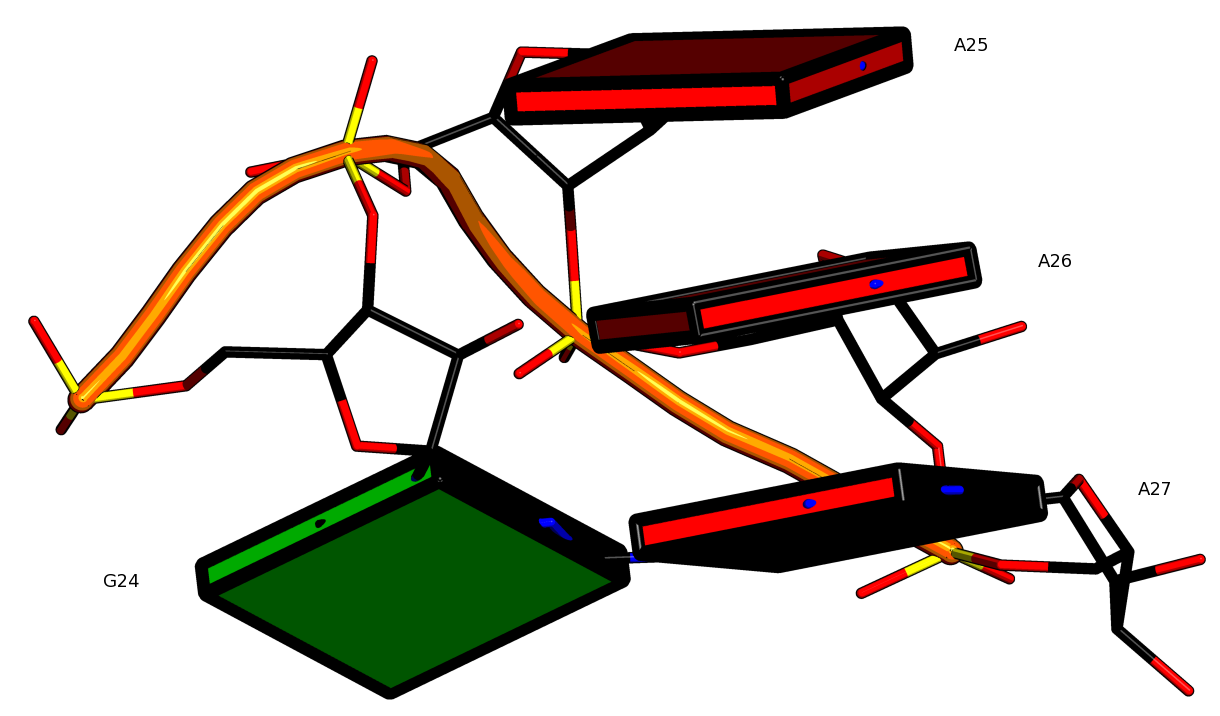
\includegraphics[angle=0]{Chapter5/gnra24.png}
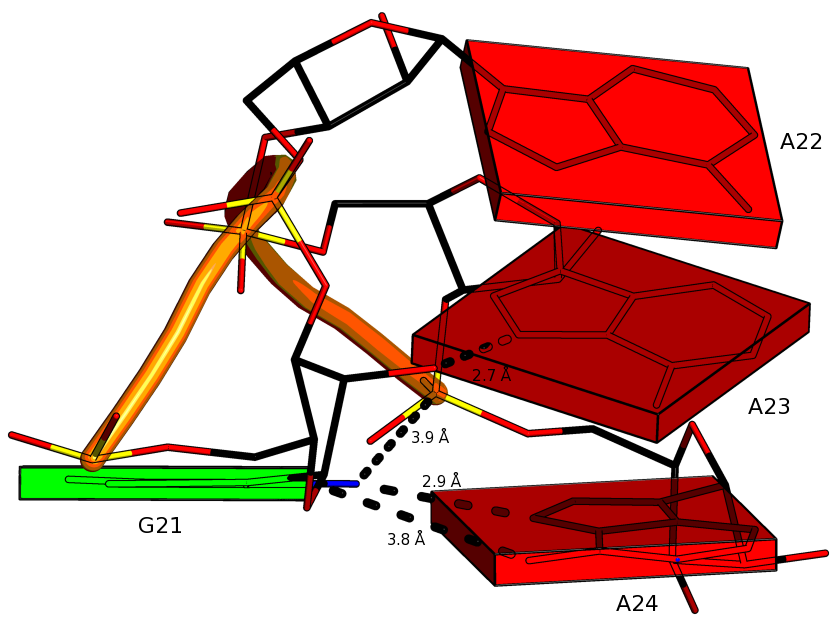
\includegraphics[angle=0, scale=0.38]{Chapter5/gnra21L2.png}
\caption{The   GNRA  tetraloop  motif   in  the   hammerhead  ribozyme
  PDB\_ID:1HMH \cite{pley1994}.  Although  not a newly recognized GNRA
  tetraloop, this motif is  positively recognized using our rigid-body
  parameters RNA motif search  program ``getMotif''. The structure was
  selected from a non-redundant list of RNA structures provided by the
  RNA  ontology consortium  (ROC)  \cite{leontis2006b}.  The  hydrogen
  bonding  interactions described  by Heus  and  Pardi \cite{heus1991}
  detected in NMR experiments are shown by black dashed lines.}
\label{fig:gnrablocks}
\end{figure}

The description of  the GNRA tetraloop motif is a  typical case of the
problem  of RNA  motif definition.   For  example, in  the context  of
sequence  alone  a  GNRA motif  would  be  one  which contains,  in  a
consecutive  manner,  the  GNRA  pattern  of bases.   There  are  GNRA
structures, however,  which are not  formed by a  consecutive sequence
but  rather   have  the  same   geometric  arrangement  of   bases  in
three-dimensional  space   as  the  sequentially   linked  GNRA  motif
\cite{lee2003, lemieux2006}.  There are also structures which have the
same geometric arrangement and sugar-phosphate backbone connections as
the GNRA tetraloop,  but do not have the same sequence  of bases as in
the UCAA,  UCAC, CAGA, and CAAC  tetraloops \cite{lemieux2006}.  These
other  sequences  which  are  geometrically  equivalent  to  the  GNRA
tetraloop motif  form non-canonical base-pairs which  are isosteric to
the sheared  G$\cdot$A base-pair.  That is, the  U$\cdot$A, U$\cdot$C,
C$\cdot$A, and C$\cdot$C  base-pairs closing the respective tetraloops
are isosteric to  the G$\cdot$A base-pair at the end  of the GNRA loop
\cite{lemieux2006}.

A  number  of  molecular  dynamics  (MD)  studies  have  explored  the
conformational   space  of   the  GNRA   tetraloop  \cite{cornell1995,
  sorin2002, spackova2010,  depaul2010}. These  studies find a  set of
conformational states  for the GNRA tetraloop motif  which are closely
related  to existing X-Ray  and NMR  structures available  through the
Protein Data Bank \cite{depaul2010, sorin2002}.  Other MD studies have
used the well known GNRA  motif conformation as the starting point for
simulation  of other  tetraloops  \cite{srinivasan1998}.  These  other
tetraloops do  not retain  a GNRA-like three-dimensional  structure in
the simulations  \cite{srinivasan1998}, but this  effect might reflect
the force  fields used in such calculations  \cite{cornell1995} do not
correctly  predict  known  tetraloops  strucutures such  as  the  GAAA
tetraloop \cite{spackova2010}.

\subsection{GNRA Motif Search Program}
We have devised  a simple algorithm, ``getMotif'', to  search for GNRA
motifs  based  on  their  base  step  parameters.   The  algorithm  is
summarized in Figure \ref{fig:getMotif}.

\begin{figure}[ht]
\centering
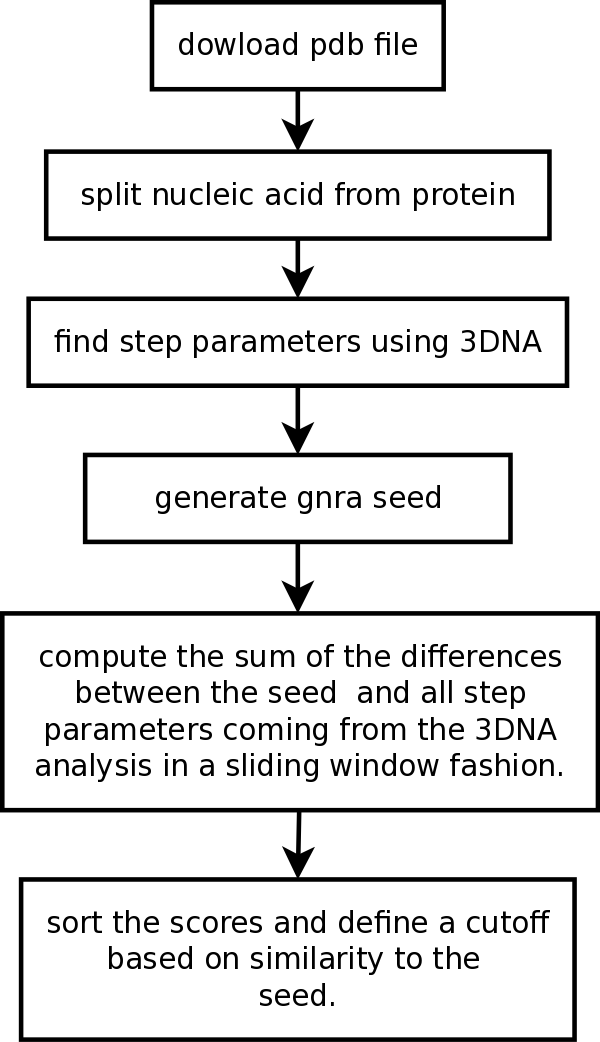
\includegraphics[angle=0, scale=0.4]{Chapter5/getMotif.png}
\caption{Simple algorithm  for GNRA motif  finding based on  base step
  parameters.}
\label{fig:getMotif}
\end{figure}
  
The algorithm  allows for any  motif seed to  be used, but for  now we
only  use the  step parameters  of the  GNRA motifs  found in  the 23S
subunit of rRNA (PDB\_ID:1FFK) by Lemieux et al. \cite{lemieux2006} as
the seed for our algorithm.   We are currently constructing a database
of  the base-step  parameters for  known  motifs, so  that our  simple
program can  be expanded to include  various known motifs  that a user
wishes to localize in an arbitrary RNA structure.

The  algorithm has  been programed  as a  simple, yet  very  fast bash
script \footnote{For  ease of use and  development a future  aim is to
  code the algorithm fully in python without compromising the speed of
  structure analysis.}  which interfaces  with three components -- one
written in  python, the  second being the  3DNA package, and  the last
written in the statistical analysis  software R.  For example, for the
large subunit  of the ribosome,  PDB\_ID:1JJ2, the program  takes 22.1
seconds to download  and analyze the whole structure  on an Intel Core
Duo of 2.13GHz with 8Gb of RAM.

The program  allows the user to  query any PDB\_ID. That  is, the user
only needs to  input in the command line of  a UNIX/LINUX terminal the
command, ``getMotif'' followed  by the PDB\_ID of the  RNA molecule of
interest.  As  a result  the user obtains  a list composed  of residue
numbers corresponding to the location of the start of the motif in the
structure,  and a  score which  stands  for how  close or  far a  four
nucleotide  sequential structure  is from  the GNRA  motif  seed.  The
advantage of  our program  over other Windows-based  motif recognition
software,  aside from  providing a  new analysis  based  on rigid-body
parameters,  is  that it  allows  for  easy  integration of  automated
scripts  for processing large  lists of  known PDB  structures without
user intervention for the analysis of every structure. For example, in
the  RNA ontology  consortium  (ROC)  meeting of  May  2009 a  reduced
dataset        of        RNA        structures        found        at:
\url{https://docs.google.com/Doc?id=dhrmkfmn_13ftpbjcgq}    was   made
available to participants with the  purpose of allowing them to search
for  RNA motifs  which would  later be  compared among  groups.  Using
Windows-based  softwares   like  FR3D  \cite{sarver2008}   it's  quite
difficult for  the user  to submit  a large job  composed of  many PDB
structures to a  queing system, or a cluster  computing server. Such a
task is made simple using getMotif.

To construct  the seed for  the GNRA motif  we extracted the  first 20
GNRA tetraloop motifs found by Lemieux and Major \cite{lemieux2006} in
the large subunit of the ribosome (PDB\_ID:1FFK) as show in Figure 3 of
their results. After computing the  base-step parameters with 3DNA for
each of these motifs, we arranged their average values in a 3 x 6
matrix $S$ where each row corresponds to one of the three steps in the
tetraloop. These average values are show in Table \ref{tab:seed}.

\begin{table}[hb]  
\begin{center}
\begin{tabular}{|c|c|c|c|c|c|c|}
\hline
Step & Shift & Slide & Rise & Tilt & Roll & Twist \\
\hline
GN & -9.77 & -1.90 & -4.93 & 71.8 & 124.0 & -57.5 \\
NR & 2.74 & -0.11 & 3.04 & 11.5 & 6.0 & 50.6 \\
RA & 1.11 & -0.20 & 3.01 & 9.5 & 6.1 & 42.4 \\
\hline
\end{tabular}
\caption{GNRA motif  seed composed of the average  base step parameter
  values for 20 GNRA motifs found in the large subunit of the ribosome
  PDB\_ID:1FFK \cite{lemieux2006}.}
\label{tab:seed}
\end{center}
\end{table}

We  then  compute  a  score  to determine  the  distance  between  all
sequences formed by  three sequential steps in a  given RNA structure,
and the GNRA  motif seed. The score is simply the  sum of the elements
of the difference matrix $X_{k}$,  where the difference is between the
base-step parameters in the GNRA seed matrix $S$ and the corresponding
parameters  for  three sequential  steps  in  each  one of  the  $k-3$
sequential 3  x 6 matrices $W_{k}$,  where $k$ is the  total number of
steps in the RNA structure.

\begin{gather}
X_{k} = |S - W_{k}| \\
\text{score}_{k} = \sum X_{m,n} 
\end{gather}  

The scores  obtained from analysis  of the large ribosomal  subunit of
the  ribosome PDB\_ID:1FFK  can be  seen in  the histogram  displayed in
Figure \ref{fig:gnrahist}.

\begin{figure}
\centering 
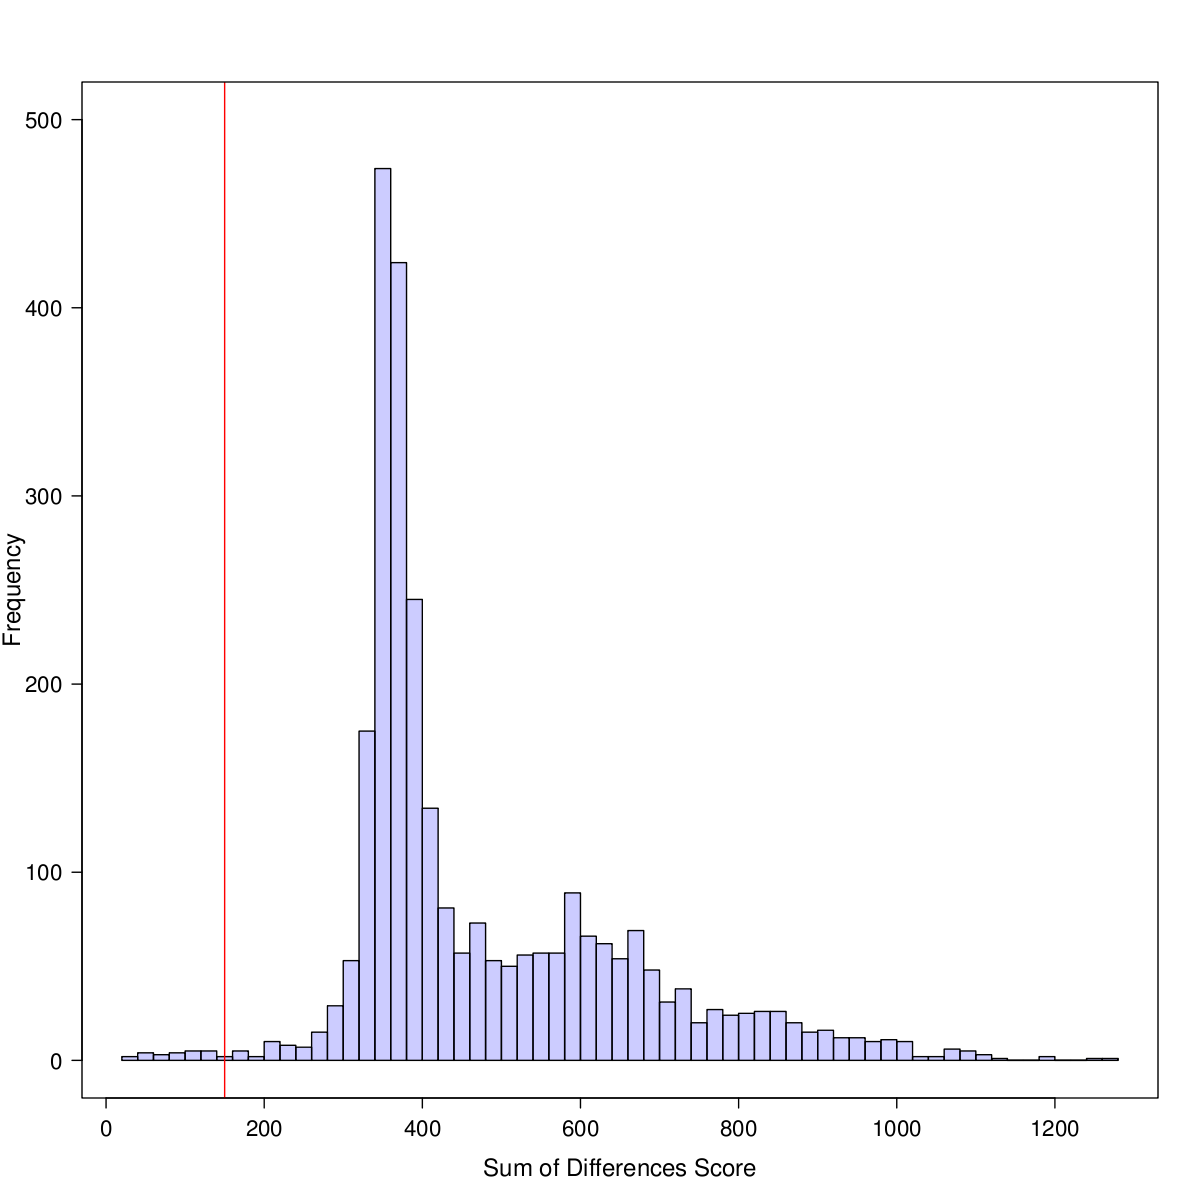
\includegraphics[angle=0, scale=0.5]{Chapter5/gnrahisto.png}
\caption{Histogram of  the sum of  differences score between  the GNRA
  seed  motif and  all  sequential tri-nucleotide-steps  found in  the
  large subunit of the ribosome PDB\_ID:1FFK}
\label{fig:gnrahist}
\end{figure}

In  this  histogram  we   see  that  the  majority  of  trinucleotides
(tristeps)  have scores  between  350-400.  These  values most  likely
correspond to tri-step sequences  with base-step parameters similar to
those  of   A-RNA-like  steps.   For   our  purposes  of   GNRA  motif
identification we want to select those steps with scores which reflect
a shorter distance  to our seed GNRA motif.  Therefore  we have used a
cutoff score of 150, which is  represented by the values below the red
vertical line in Figure \ref{fig:gnrahist}.

Application of our program to  the list of 355 RNA structures provided
by the  ROC, with a  cutoff value of  150 finds \footnote{The  time it
  took  to search  for GNRA  tetraloop  motifs candidates  in the  355
  structures was 7  minutes and 29 seconds} 75  of these structures to
have at  least one GNRA  3D motif candidate,  and a total of  211 GNRA
motif  candidates.  The  list of  all  identified motifs  in these  75
structures including the parameters at the first step, is presented in
Table  \ref{tab:gnrascores}, which  includes an  additional  check for
consistency  in the  next  to last  column.  The latter  entry is  the
overlap or the ring atoms of the first two base pairs of the tetraloop
which showed  zero in the described  structures.  We see  that 67\% of
the  identified  GNRA motif  candidates  start  with  a GN  step,  and
interestingly that, almost one third  (27\%) of the first steps are UN
steps, and  that a few of the  identified motifs start with  AN and CN
dimers.

To  further  analyze  the  results  of  the  motifs  identified  using
``getMotif'',  we   focused  attention  on   the  ribosomal  structure
(PDB\_ID:2J01) that  is included in the  ROC list.  As can  be seen in
Table   \ref{tab:gnrascores}  for  the   2J01  entries,   the  program
recognizes twenty  GNRA tetraloop motif  candidates, all of  which are
,in fact, tetraloops,  of these 13 conform to  the GNRA sequence, five
start with UN,  one starts with A  and one with C.  When  we align the
candidate GNRA motif sequences using  the reference frame of the first
two  bases,  we  see that  they  fall  into  two main  groups  (Figure
\ref{fig:groupsB}), one  with about eleven members and  the other with
seven members.  The  two remaining structures fit well  with the first
two steps, of both  groups I and II, but do not  fit well on the third
step in  either group.  Group  I, which is  colored in blue  in Figure
\ref{fig:groupsB} is closer to the  common GNRA motif. Group II, which
is  colored in  red  folds close  to  the common  GNRA  motif but  the
residues  which would  form  the terminal  G$\cdot$A  base-pair are  a
little  too   far  from  each   other  to  form  a   hydrogen  bonding
pattern. This variation stems from a  large rise in the last step. The
first two  steps are  very closely related  in every  case, suggesting
that there  is a subtle switch  between the tetraloop  and a pentaloop
conformation, governed by the rise in the last step.

\begin{figure}
\centering 
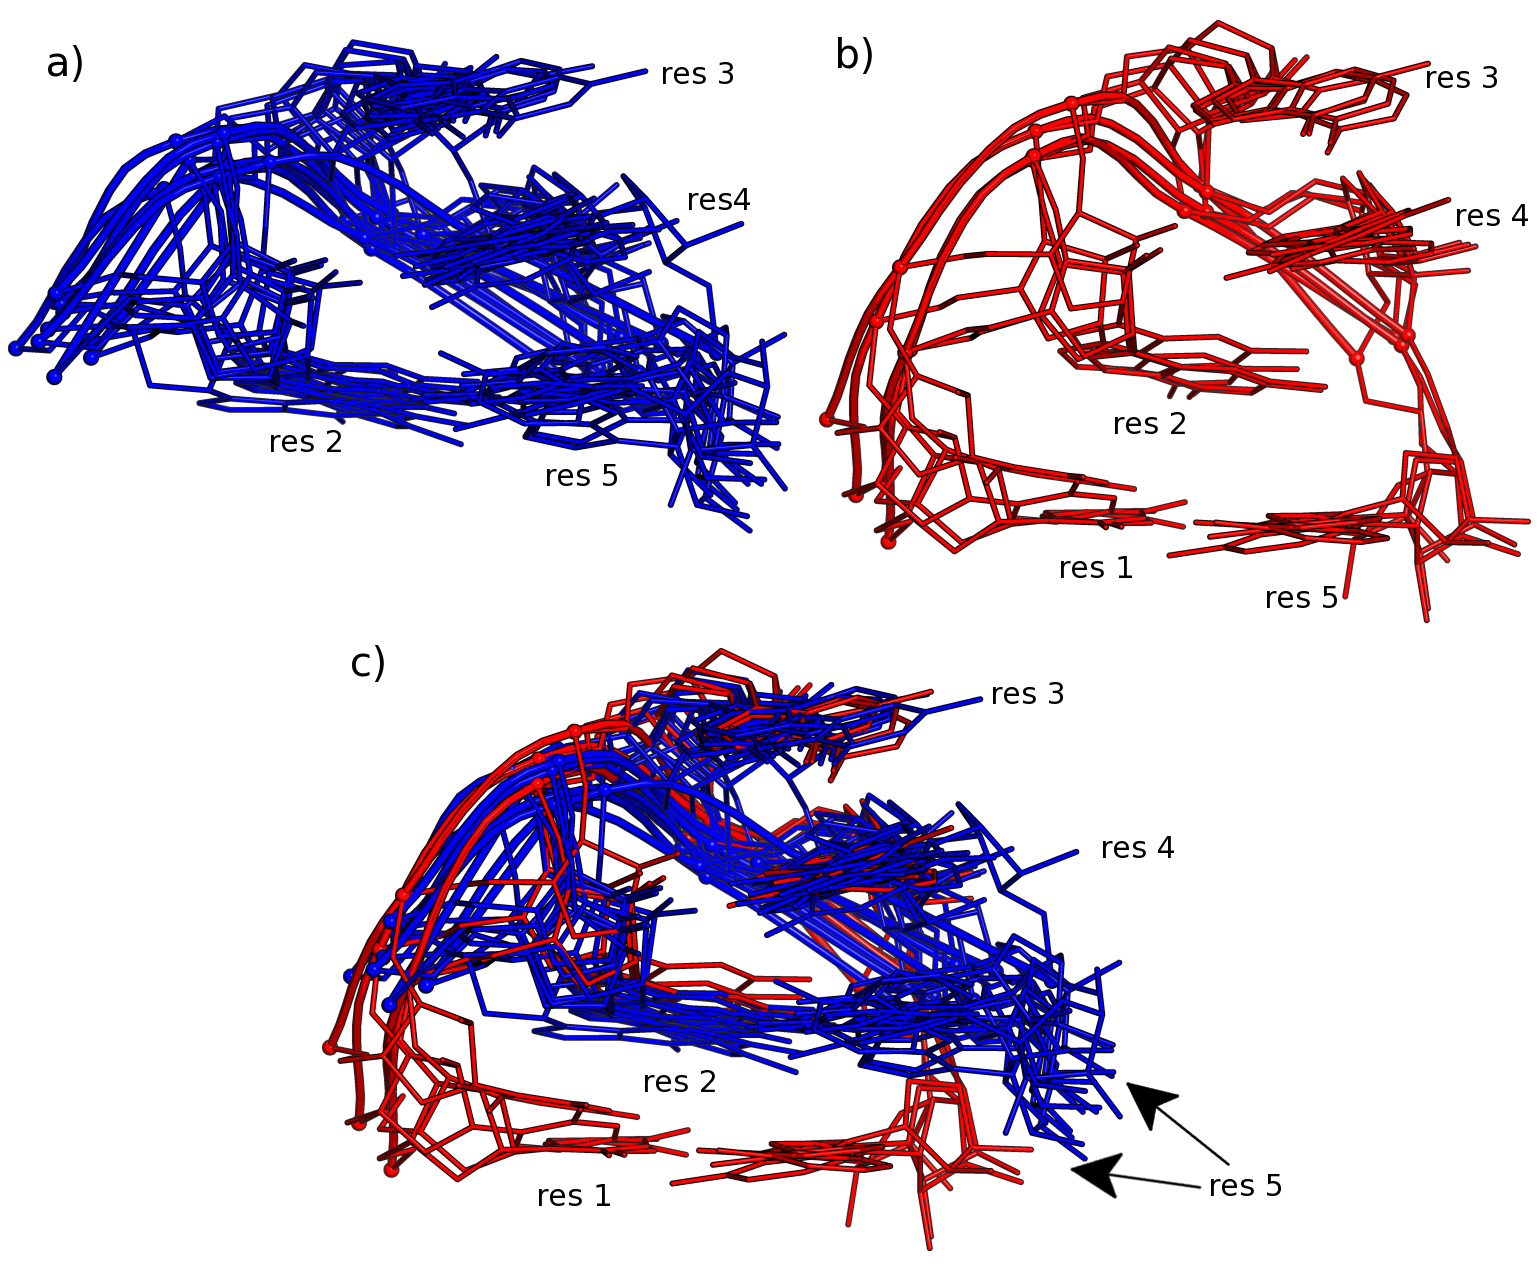
\includegraphics[angle=0, scale=2]{Chapter5/groupsB.png}
\caption{Two main groups of  tetranucleotide structures related to the
  GNRA  motif  identified   using  ``getMotif''.  All  structures  are
  superimposed  using  the  refence  frame between  residues  two  and
  three. In a)  Group I structures which are drawn  in blue, are close
  to a  typical GNRA motif.  The  Group II structures in  b) which are
  drawn in red  are closer to a pentaloop.  The steps between residues
  two and three, and three and four are common to the two groups as is
  clearly seen from  the superposition of both groups  in c).  Residue
  two  from Group  II is  commonly found  forming a  sheared G$\cdot$A
  base-pair  with   a  sequentially   distant  base.   This   type  of
  interaction, which maintains the GNRA motif geometry and is called a
  lonepair  triloop  \cite{lee2003}  has  been previously  found  from
  sequence covariation analyisis.}
\label{fig:groupsB}
\end{figure}

Interestingly some of  the GNRA candidates identified in  Group II are
part    of   a    highly   symmetrical    extended    "kissing"   loop
interaction. These  can be seen  in Figure \ref{fig:terts}  where they
are  superimposed, and  shown  in their  original  orientation in  the
ribosome. This type of interaction  is part of what has been described
as the lonepair triloop motif found by sequence covariation techniques
\cite{lee2003}.  The GNRA motif  candidates found by ``getMotif'' have
been named recently by Nasalean et al. \cite{nasalean2009} as internal
and composite motifs.  In our  case the GNRA motif candidates in Group
I correspond to the internal motifs, and the Group II candidates
correspond to the composite motifs.

\begin{figure}
\centering 
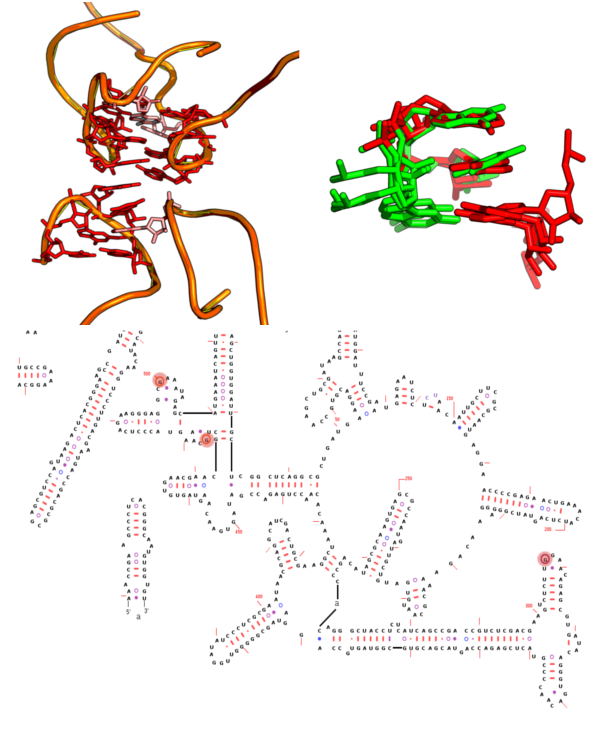
\includegraphics[angle=0, scale=2.5]{Chapter5/lonepairtlooptert.png}
\caption{Subset   of   the  Group   II   structures  identified   with
  ``getMotif'',  which  correspond   to  the  lonepair  triloop  motif
  identified by Gutell and collaborators \cite{lee2003}.  In the upper
  left  corner of  the figure  sequentially distant  adenine  drawn in
  pink,  forms  a  sheared  G$\cdot$A base-pair  with  the  identified
  GroupII structure, which is drawn in red.  In the upper right corner
  of the figure the three  lonepair triloop motifs, or structural GNRA
  motifs are superimposed  in the reference frame of  residues two and
  three. In the lower portion of  the figure the location of the first
  residue of  the identified GNRA structural motifs  is highlighted in
  pink on top  of the secondary structure of the  large subunit of the
  ribosome, taken from Gutell Lab's website \cite{cannone2002}.  }
\label{fig:terts}
\end{figure}

Of the three steps which make  up the GNRA tetraloop, the first one is
the step farthest  away from a typical A-RNA-like  base-step.  We plot
the step-parameter  values for this  first step in the  scatterplot in
Figure \ref{fig:scattergnra}.  It is clear from  this scatterplot that
these  steps  constitute  a  well  defined  region  in  the  space  of
rigid-body step parameter configurations  for the large subunit of the
ribosome.

\begin{figure}
\centering 
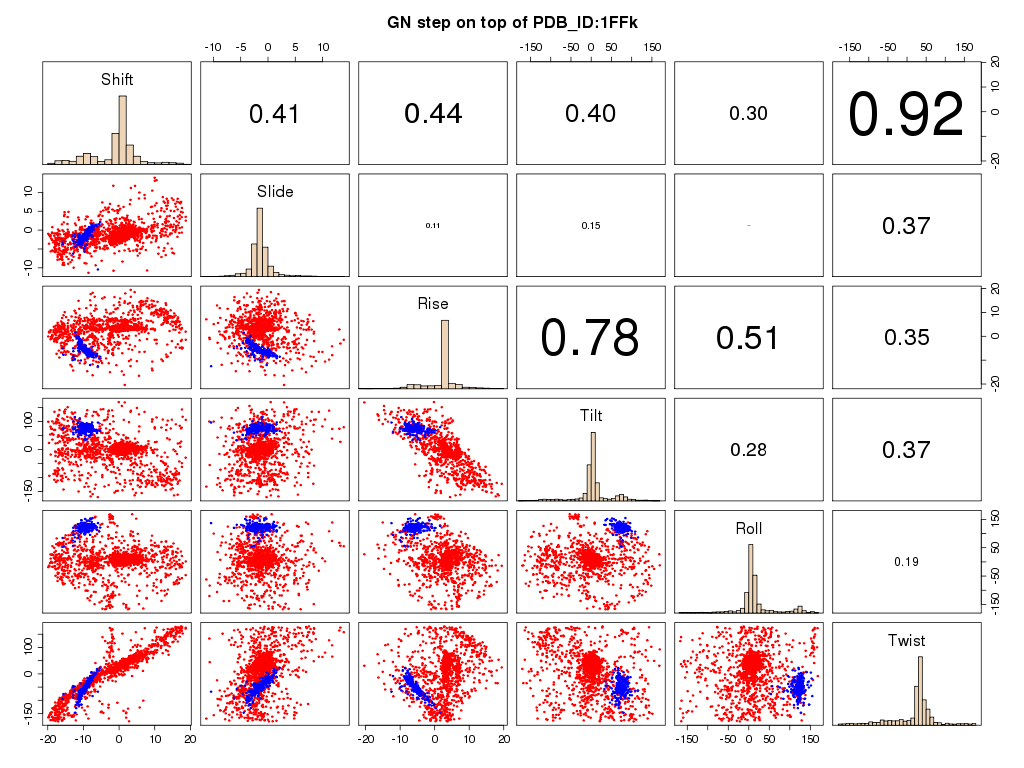
\includegraphics[angle=90, scale=0.5]{Chapter5/GNRAin1ffk.png}
\caption{Scatterplot  of  base-step parameter  values  for GNRA  motif
  candidates identified in a list given by the ROC, against a backdrop
  of the range of values  for the step-parameters in the large subunit
  of the ribosome PDB\_ID:1FFK.}
\label{fig:scattergnra}
\end{figure}

%\section{Canonical "Noise"}
%To be able to say anything about motifs it's crucial to get rid of the
%"noise" which is given by the canonical base-pair steps.
%One would think that perhaps  the X3DNA-Parser of Dr. Yurong Xin could
%help  in the  task, but  then, it  can't, because  it's based  on what
%base-pairs  have  been found,  therefore,  it  tells  me about  single
%stranded interactions,  it doesn't tell  me about bases which  are not
%forming interactions and are alone.

%\subsection{3DNA-Parser}
%We started by using Dr. Yurong Xin's 3DNA-Parser hoping that the
%description of the enclosing base pair in the loop, that is, the
%sheared G$\cdot$A, would have a characteristic signature.
%We found that such is not the case. We know from Major et
%al. \cite{lemieux2006} that there should be at least 21 GNRA tetraloops
%in the 23S subunit of rRNA. We used the G2696 N2697 R2698 A2699
%tetraloop as a seed (as can be seen in Figure 1.1) and found out
%that according to Dr. Xin's helical classification the enclosing G is
%classified as $S_{hq}$ and A is classified as $H_{e}$. 

%We then searched all such instances for G$\cdot$A base-pairs and we
%found seven hits, but none were in fact GNRA tetraloops.

%\subsection{Overlap Scores} 
%We  clustered the  overlap  values  impossing a  cutoff  of values  of
%[1-8]. Since a large amount of overlap values are exactly zero (33\%),
%so, without the cutoff the zero values "overshadow" the data.
%\begin{figure}[htbp]
%\centering 
%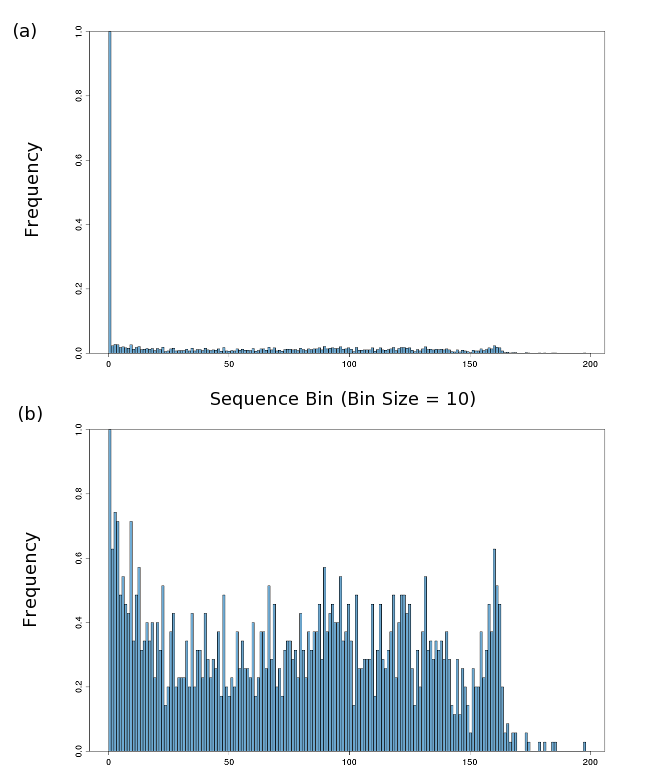
\includegraphics[angle=0, scale=0.8]{Chapter5/histocompare.png}
%\caption{Normalized  histograms showing  the  distribution of  overlap
%  values  in the  23S subunit  or \textit{Thermus  Thermophilus} rRNA,
%  PDB-ID:1jjk.  In  histogram (a)  all  values  are  included, but  in
%  histogram (b) only values greater than zero are included. Notice the
%  high preponderance  of zero  values, exactly 897  out of a  total of
%  2705.}
%\end{figure}
%For this case we obtain the dendrogram shown in Figure 1.2.
%\begin{figure}[htbp]
%\centering 
%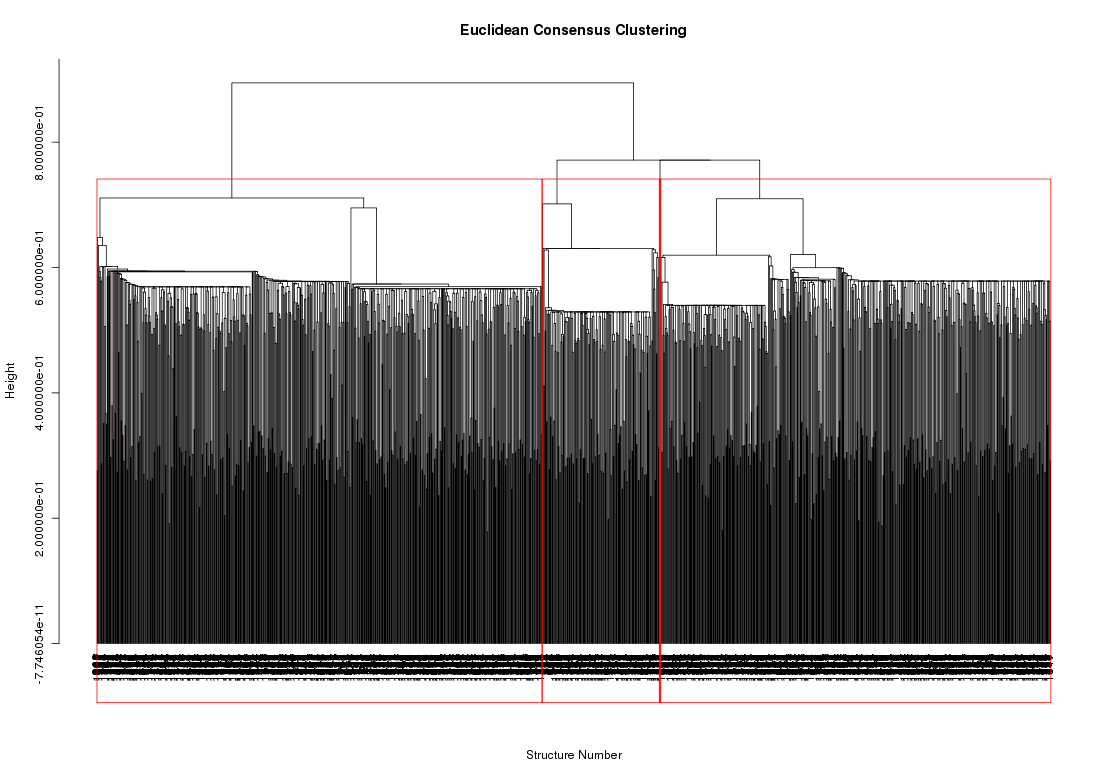
\includegraphics[angle=90, scale=0.6]{Chapter5/eucli_cons.png}
%\caption{Dendrogram for consensus clustering  of overlap scores in the
%  ribosome.  Zero values filtered out and remaining data normalized.}
%\end{figure}

%The next  step in this analysis  will be to find  the structures which
%correspond  to this  clusters  and superimpose  and  align them  using
%Kabsh's algorithm to be able to determine their RMSD's.

%Many people  start their  RNA Motif identification  and classification
%algorithms by splitting  RNA structures into what is  helical and what
%is not,  and then  finding interactions between  these two  groups. We
%believe that  we could do  a similar exercise  with 3DNA by  using the
%scalar  product   of  helical  axis  vectors  and   once  helical  and
%non-helical regions are  found we might be able to  use 3DNA Parser to
%look for characteristic interactions.

%\section{Triplets on RNA (comparison to Laing et al.)}

\section{Conclusions}

We  answer  the questions  at  the begining  of  this  chapter in  the
following way:

\begin{enumerate}
\item{\textbf{Q.}  Can   the  geometric  rigid-block   description  of
  base-pairing  and base-stacking  solve the  problem of  defining RNA
  structural motifs?}
\item{\textbf{A.}  The  problem of  defining RNA structural  motifs is
  clearly  more  complicated  than  what  can  be  understood  by  any
  structural  research  methodology  alone,  say,  just  the  backbone
  methodology, or  the all atom  analysis methodology.  We  have shown
  that the  rigid-body parameter view  of RNA can easily  automate the
  process of motif searches in  RNA atomic structures, and it helps in
  the rigorous structural description  of motifs, therefore we believe
  that  this type  of characterization  should not  be ignored  by the
  community and included in ontological efforts such as the ROC one.}
\item{\textbf{Q.} Can we use quantities derived from the 3DNA software
  package to make and automatic search for a known motif, for example,
  the GNRA tetraloop motif, and perhaps find unknown motifs?}
\item{\textbf{A.} Yes. by defining seeds from known motifs we can find
new motifs in  the boundaries of known ones  via base-pairs steps. But
we  can also  do  other,  yet simpler,  not  as ``precise''  searches,
e.g. by clustering  the results of base overlaps.  Other searches have
not  been explored  but could  also be  useful, for  example exploring
helical  parameters like x-displacement,  y-displacement, inclination,
tip.} 
\end{enumerate}

\bibliography{biblio}

